%!TEX root = ../report.tex

\begin{document}
    \chapter{Methodology}

     \section{Pipeline Workflow: 2D Binary Lane Segmentation}
        \subsection{Architecture Overview}
        We have utilized the dual-stage architecture proposed by \cite{guo2020gen} to obtain 3D lane points, where the output from the first stage is binary lane segmentation. And authors have not explored the efficacy of more complex architecture for binary 2D lane segmentation on 3D lane detection results. So we experimented with some mentioned approaches in section 3.1 for the same. In this section, we will briefly discuss the neural network architecture for the binary 2D lane segmentation that we have experimented with in this work. 
        
        Originally \cite{guo2020gen} have utilized ERFNet\cite{Romera2018ERFNetER} based network to obtain binary segmentation which is an auto-encoder based network for the first stage. For that we conducted a comparative evaluation with the existing pre-trained models using CondLaneNet\cite{DBLP:journals/corr/abs-2105-05003}, SCNN\cite{pan2018SCNN}, RESA\cite{DBLP:journals/corr/abs-2008-13719}, Ufld \cite{DBLP:journals/corr/abs-2004-11757}, LaneATT\cite{https://doi.org/10.48550/arxiv.2010.12035} which we will talk about in the later sections. As we have discussed in section 3.1 that there is more scope in extracting more meaningful features for segmentation-based 2D lane detection and to facilitate the 3D lane detection we need 2D binary lane segmentation as an intermediate output. so explored two segmentation based approaches as mentioned above SCNN\cite{pan2018SCNN}, RESA\cite{DBLP:journals/corr/abs-2008-13719}. Both of these approaches are using semantic segmentation to predict 2D lane line points where the input to the network is a monocular image. But in our case we need binary segmentation as the output, so we modified the existing approaches to work for 2D binary lane segmentation.    
        
           \begin{figure}[h]
    \centering
    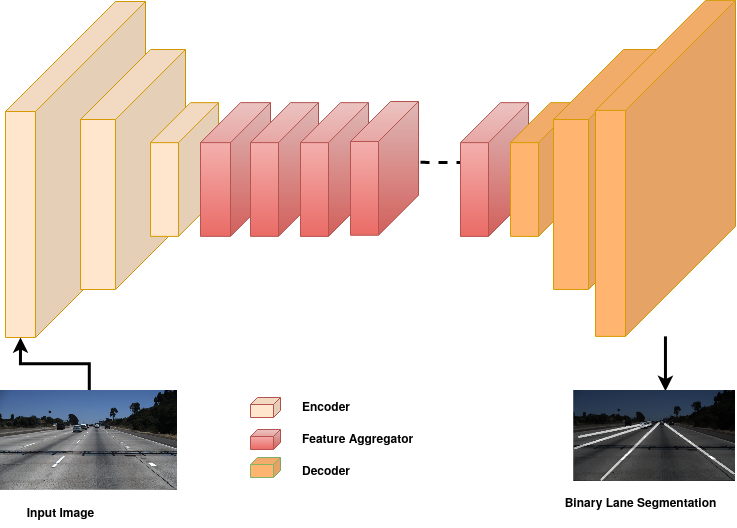
\includegraphics[width=12cm, height=7cm]{images/2dlane_pipleline.png}
    \caption{2D Binary Lane segmentation Pipeline}
    \end{figure}
        
        Figure 4.4 represents the pseudo architecture for the 2D binary lane detection module. This is an auto-encoder-based pipeline where we have used ResNet \cite{DBLP:journals/corr/HeZRS15} based network for initial feature encoding and later utilized the feature aggregation modules proposed by SCNN\cite{pan2018SCNN} and RESA\cite{DBLP:journals/corr/abs-2008-13719}. In the end, we have experimented with two types of decoders for upsampling the extracted features as it is a dense prediction task we need the output to be of the same spatial size as the input. Initially, we used the simple decoder proposed by SCNN\cite{pan2018SCNN} which uses bi-linear interpolation to upsample the feature maps, later we experimented with the Bilateral Up-sampling Decoder (BUSD) proposed by RESA\cite{DBLP:journals/corr/abs-2008-13719}. So we trained our 2d binary lane segmentation pipeline using mix and match of the above-mentioned encoder, decoder, and feature aggregation modules.
        
        \subsection{Loss Functions Used}
        The task of semantic segmentation is considered a dense prediction task, as the size of predictions and input remains the same. The model predicts for every pixel a class label to which it belongs. Binary segmentation can be seen as a subset of the task of semantic segmentation where instead of predicting multiple class labels we generally try to predict the foreground and background. The foreground in our case can be the lane lines and the background is the remaining entities in a driving scenario.
        Binary segmentation or semantic segmentation in general takes as an input an RGB image which can be of shape $(N,C,H,W)$ where $N$ is the batch size, $C$ the number of channels ie. in our case 3 representing $R, G, B$ and $H,W$ is the spatial size of the respective image. In case of binary segmentation the predictions are generally of the shape of $N,H,W$ or $N,C,H,W$ which later decides the choice of objective function used to train the pipeline. Binary Cross Entropy(BCE) is used in the case when the output is of the shape of $N,H,W$ as in the later case Cross Entropy is utilized.
        
                 \begin{figure}[h]
    \centering
    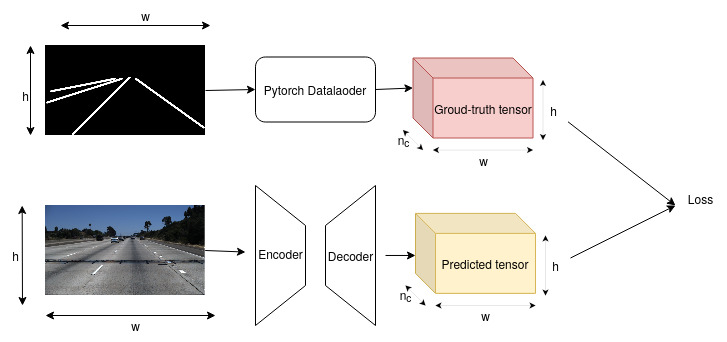
\includegraphics[width=13cm]{images/2d_dataflow_loss_computation.jpg}
    \caption{Data flow for loss computation for 2D binary lane segmentation pipeline. $w$ and $h$ are the spatial width and height of the image tensors and $n_{c}$ represents the number of classes.}
    \end{figure}
        
        \subsubsection{Cross Entropy Loss}
        Cross Entropy is generally employed to measure the difference between two probability distributions.
        \begin{equation}
        L_{CCE} = -\frac{1}{N}\sum_{i=1}^{N} \sum^{M}_{j=1}y_{i,j}\cdot log(p_{i,j})
        \end{equation}
        
        where $p_{i,j}$ is the prediction for each class and $y_{i,j}$ is the target values for each class. $y_{i,j}$ is represented as a one-hot encoded matrix of ground-truth labels which is represented in the form of different channels per each class. The rows and columns of each channel are either 0 or 1 depending upon the location of pixel-wise class labels. 
       
        \subsubsection{Focal Loss}
        Focal loss can be seen as an extended version of cross entropy where the objective function will penalize the hard samples than the easy samples and to achieve that a regulating term is added to handle the class imbalance problem.
        \begin{equation}
            Cross Entropy = - \sum^{i=n}_{i=1}Y_{i}log_{b}(p_{i})
        \end{equation}
        where $Y$ is the ground-truth label and $p$ is the predicted probability.
        
        \begin{equation}
            Focal Loss = - \sum^{i=n}_{i=1} \alpha_{i}(1-p_{i})^{\gamma} log_{b}(p_{i})
        \end{equation}
        
         when $\gamma = 0$, Focal Loss is equal to Cross Entropy Loss. 
        
        \subsubsection{Dice Loss}
        Dice Similarity Coefficient(DSC) is a popular loss function that is used for the task of semantic segmentation to counter the problem of class imbalance. DSC is quite similar to Intersection over Union(IoU). Like IoU, Dice Similarity Coefficient(DSC) is used to compare the predicted segmentation mask and the corresponding ground truth. In simpler terms, DSC is 2 times the area of overlap between the segmentation mask and the ground-truth mask divided by the total number of pixels in both the prediction and ground-truth mask.
        
        \begin{equation}
            DC = \frac{2TP}{2TP + FP + FN} = \frac{2|X \cap Y|}{|X| + |Y|}
        \end{equation}
    where $TP$ are the true positives $FP$ false positives and $FN$ false negatives.  
        
        \begin{equation}
            L_{dice} = 1 - DSC
        \end{equation}
        
        \subsection{Evaluation Metrics}
        All the utilized datasets have their evaluation metrics and even the authors have released the script for bench-marking the results and the evaluation criteria proposed by them only rely on penalizing the predictions based on predicted 2d lane line points. As in our case, we are not interested in predicting lane line points rather our 3D lane detection module relies on 2d binary lane segmentation masks as intermediate output. So we have used IoU (Intersection-over-union) or Jaccard Index to evaluate the trained models. IoU is a commonly used evaluation metric for image segmentation which is effective. In Simple terms, IoU calculated the area of overlap between the predicted segmentation mask and the ground truth divided by the union of the predicted segmentation mask and ground truth.
        
         \begin{figure}[h]
    \centering
    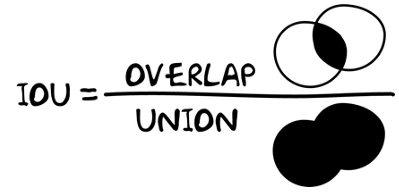
\includegraphics[width=7cm, height=4cm]{images/IOU.png}
    \caption{(IoU)Intersection-Over-Union \footnotemark}
    \end{figure}
    \footnotetext{\url{https://towardsdatascience.com/intersection-over-union-iou-calculation-for-evaluating-an-image-segmentation-model-8b22e2e84686}}
        
        \subsection{Implementation Details and Other Design Choices}
        We have utilized three datasets for training the 2D binary lane segmentation pipeline. The first dataset is called TuSimple lane detection benchmark\cite{Tusimple}, as discussed in section 3.3.3 it is a simple dataset consisting of normal highway driving. On the other hand, we also use a more complex and much larger dataset compared to the previous one like CULane\cite{pan2018SCNN} which contains 55 hours of driving and contains different driving scenarios as discussed in section 3.3.3. We have also trained the 2D binary lane segmentation with the Apollo Synthetic dataset\cite{guo2020gen} by utilizing the semantic segmentation labels provided in the dataset. We have conducted several experiments on the above-mentioned datasets in terms of usage of different objective functions (dice loss, categorical cross-entropy loss, focal loss), different variants of the network using mix and match of the above-discussed encoder, decoders, and feature aggregators. The input image is resized to $(360,480)$ and normalized using Imagenet\cite{deng2009imagenet} mean and standard deviation values. Adam\cite{Kingma2015AdamAM} with weight decay $1e-4$ is used as an optimizer to train our models. $0.001$ is chosen as an initial learning rate and on top of that, we have used ReduceLROnPlateu \footnote{\url{https://pytorch.org/docs/stable/generated/torch.optim.lr_scheduler.ReduceLROnPlateau.html#torch.optim.lr_scheduler.ReduceLROnPlateau}} as the learning rate scheduler with $0.75$ as learning rate reduction factor, $3$ as patience factor denotes the number of epochs to wait when the learning rate has to be reduced if there is no improvement in loss, $1e-6$ as the lowest learning rate managed by the scheduler. All the models are trained with the batch size of $8, 16$ but we have only reported the results with batch size $8$, and training is carried for $60$ epochs. During training, the model is evaluated at every epoch and the results are visualized qualitatively and quantitatively using wandb \footnote{\url{https://wandb.ai}}.
        
    %---------------------------------------------------------------- After here must start 3D lane detection section%   
        
        \section{Pipeline Workflow: 3D Lane Detection }
        Before delving into the approaches that we have used to obtain 3D lane line points we need to understand how a 3D lane is represented with respect to the ego vehicle frame of reference and the anchor-based representation of the 3D lane curve.  
        
        \subsection{3D Lane Geometry}
        In this section, we will introduce the geometric representation of lanes in 3D space, image plane, and birds-eye view via the means of the transformation from one space to another. 
        
         \begin{figure}[h]
    \centering
    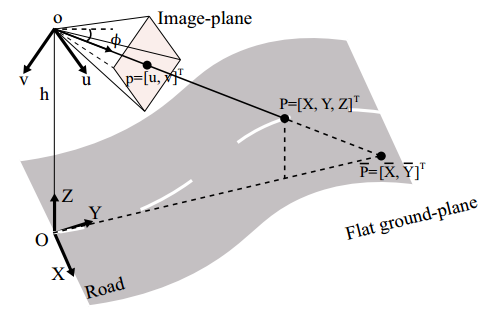
\includegraphics[width=9cm, height=5cm]{images/3d_lane_geometry.png}
    \caption{Geometric representation of lane point in 3D world space, image plane and virtual top view \cite{DBLP:journals/corr/abs-2112-15351}}
    \end{figure}
    
    In the above figure the point $\textbf{P} =[X, Y, Z]^{T}$ is in 3D space and when it is projected onto the image plane it is defined by $\textbf{p} = [u, v]^{T}$. Birds-eye-view can be seen as the projection of point $\textbf{P}$ from 3D space to a flat ground plane, where $Z=0$. $\textbf{O}$ is the origin of the 3D space which is obtained by projecting the origin of camera center $\textbf{o}$ onto the flat ground plane with $Z = 0$. The focal length and other intrinsic parameters of the camera are fixed, whereas the orientation of the camera in terms of camera height \textbf{h}  and camera pitch \textbf{$\phi$} is fixed or sometimes it is predicted from the network. 
    
    Using geometric transformation and homography as discussed above we can project points in 3D space to the virtual flat ground plane. As per figure 4.1, we can say that the point \textbf{P} it projection on the image plane and flat ground plane, all lies on the same ray and this co-linear relationship will hold even if when there are downhill scenarios where $Z<0$. 
    
      \begin{figure}[h]
    \centering
    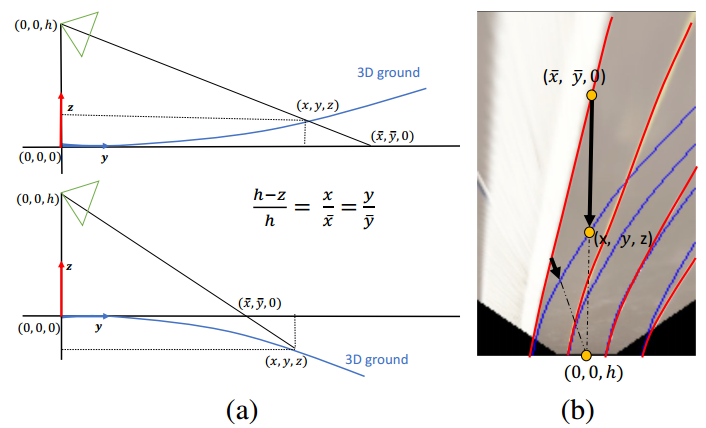
\includegraphics[width=9cm, height=5cm]{images/collinear_3dlane.png}
    \caption{Another view of the co-linear relationship between the 3D lane points $(x,y,z)$, its projection on virtual top view $(\overline{x}, \overline{y},0)$ and camera center $(0,0,h)$ \cite{guo2020gen}}
    \end{figure}

    Therefore we can obtain a relationship between the points from the 3D world to the virtual top view as :
    \begin{equation}
        \frac{h-z}{h} =\frac{x}{\overline{x}}=\frac{y}{\overline{y}} 
    \end{equation}
    
    using the above formulation we can represent this transformation from 3D world space to virtual top view as \textbf{$\overline{P} = GP$}, where \textbf{G} is the transformation matrix. Similarly, a point \textbf{$\overline{P}$} can be projected onto the image plane as $\textbf{p}$ using homography which is also discussed in section 2.2. and this can be represented as: 
    \begin{equation}
       \begin{bmatrix}\overline{u}  \\\overline{v} \\ \overline{z}\end{bmatrix} = \begin{bmatrix} f_{x} & 0& c_{x}  \\0 &f_{x} & c_{y} \\ 0 & 0 & 1     \end{bmatrix}\begin{bmatrix} 1 & 0& 0  \\0 &cos(\phi+ \frac{\theta}{2}) & h \\ 0 &cos(\phi+ \frac{\theta}{2}) & 0     \end{bmatrix}\begin{bmatrix}\overline{X}  \\\overline{Y} \\ 1\end{bmatrix}
    \end{equation}

    Here, \textbf{$\widetilde{p}$} $= (\widetilde{u}, \widetilde{v}, \widetilde{z})$ and  \textbf{$\widetilde{P}$} $= (\overline{X},\overline{Y},1 )$ are represented in the form of homogeneous coordinates, therefore $u = \frac{\widetilde{u}} {\widetilde{z}} $ and $v = \frac{\widetilde{v}} {\widetilde{z}} $. Similar as above this can be represented as \textbf{$\widetilde{p} = H\widetilde{P}$}, where H is the homography transformation matrix. 
    
     \subsection{3D Lane Anchor Representation}
    Some of the approaches used in this work are predicting 3D lane line points in the form of anchors and even the ground-truth points are also converted in the form of anchors as target tensors to the network.  As per the 3D lane geometry discussed above, x is the lateral axes and Y is the forward axes with respect to a scene. These anchors are generally predefined on the basis of equally spaced distances in x and y directions. 
    
     \begin{figure}[h]
    \centering
    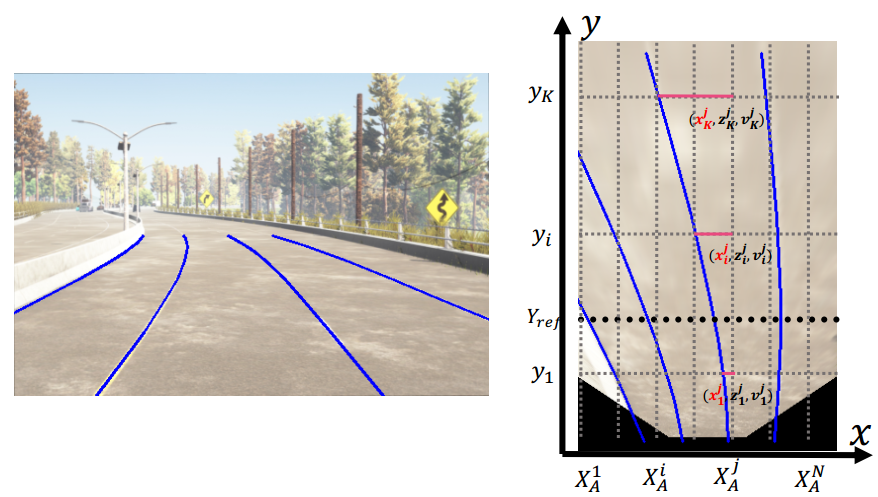
\includegraphics[width=9cm, height=5cm]{images/anchor_3Dlane.png}
    \caption{Lane anchor representation \cite{guo2020gen}}
    \end{figure}
    
    As per figure 4.3, there exist N lane anchors (Vertical lines) in terms of N equally spaced position in X-direction ($X^{i}_{A}$)$^{N}_{i=1}$. The position of anchors in the y-direction can be equally spaced or based on certain distances in the forward direction. Therefore a 3D lane line in this can be represented by an anchor $X^{i}_{A}$ where each anchor contains $3*K$ attributes. K is the number of steps in the y-direction. So at each step $(Y_ref)$ ground-truth lane anchor attributes ($\overline{x}^{i}_{j},z^{i}_{j},v^{i}_{j}$)$^{K}_{j=1}$ are calculated by associating it with the closest distance in x-direction. $\overline{x}^{i}_{j}$ are the horizontal offsets, $v^{i}_{j}$ is the visibility vector for every lane point.  In the later sections, we will talk about the approaches that we have experimented with to obtain 3D lane line points. 
        
%--------------------------------Approach 1 starts from here::%        
        \subsection{Approach 1: GenLaneNet\cite{guo2020gen}}
        
        \subsubsection{Model Architecture Overview}
        Initially, we utilized the dual-stage architecture proposed by \cite{guo2020gen} to obtain 3D lane points, and later this dual-stage way of architecture is used in our proposed 3D lane detection pipeline. In this section, we will introduce the network architecture proposed by GenLaneNet\cite{guo2020gen} in detail and explain how we have utilized it for our initial experimentation for obtaining 3D lane line points.
        
         \begin{figure}[h]
    \centering
    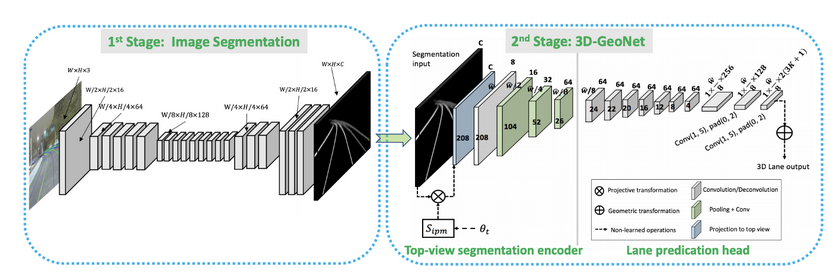
\includegraphics[width=13cm]{images/GenLaneNET.png}
    \caption{Network architecture of Gen-LaneNet \cite{guo2020gen}}
    \end{figure}
         
         Here authors have represented the 3D lane lines in the form of anchors and have utilized this representation to predict 3D lane line points by using a dual-stage network. Authors have chosen this dual pathway approach on the fact that encoding 3D lane geometry is a different task from encoding features from the image. Therefore, instead of predicting camera height and camera pitch, the ground-truth values are used for obtaining all the geometric transformations. 
         The first stage is responsible for extracting features from the input monocular image and performing a binary segmentation task on the image to obtain a binary lane segmentation mask. This obtained binary lane segmentation mask is this used as an input for the next stage of the pipeline which is responsible for predicting the 3D lane line points in the form of anchor-based representation. As described in section 4.2.2 each anchor defines a 3D lane line by 3*K values as ($\overline{x}^{i}_{j},z^{i}_{j},v^{i}_{j}$)$^{K}_{j=1}$. The ground truth target lane anchors are generated by taking the 3D lane line points which are in ego vehicle coordinate frame to virtual top view.
         
         The output from the image segmentation stage is processed by a top view segmentation encoder which uses projective transformation and projects it into the top view which is further processed by a series of convolution layers to encode features from top view binary segmentation. After that, a lane prediction head predicts 3D lane line points in terms of anchor representation. The predicted anchors are in top-view which can be further transformed into 3D lane line points in the ego-vehicle frame by using geometric transformation. This dual-stage network makes the pipeline flexible in terms of using complex binary segmentation solutions and makes it affordable as we don't need more real-world 3D lane line labels in various driving scenarios.
        
        
        \subsection{Experimental Setup: Approach 1}
        
        
            \subsubsection{Loss Computation}
            While training, the pipeline takes as an input an RGB image and predicts an anchor-based representation of 3D lane lines which is discussed in section 4.2.2. The ground-truth 3D lane points are projected in virtual top-view and the anchors are calculated in terms of different y-positions $\left\{ y_{i} \right\}^{k}_{j=1}$ by associating them with the closest anchors at that particular $Y_{ref}$. Loss function for the predicted anchors $\hat{X}_{A}^{i}$ and the ground-truth anchors $\hat{X}_{A}^{i}$ =$ \left\{(\hat{x^{i}_{t}},\hat{z^{i}_{t}},\hat{v^{i}_{t}},\hat{p^{i}_{t}})\right\}_{t\in\left\{c,l\right\}}     $ is defined as: 
            
            \begin{equation}% 
\mbox{\fontsize{15}{21.6}\selectfont\( %
 \begin{array}{l}
                l = - \sum_{t\in\left\{c,l\right\}} \sum ^{N}_{i=1}(\hat{p}^{i}_{t} logp^{i}_{t} + (1-\hat{p}^{i}_{t})log(1-p^{i}_{t}) )   \\ 
                +  \sum_{t\in\left\{c,l\right\}} \sum ^{N}_{i=1}\hat{p}^{i}_{t}\cdot(\parallel \hat{v}^{i}_{t} \cdot (x^{i}_{t} - \hat{x}^{i}_{t}) \parallel_{1} + \parallel \hat{v}^{i}_{t} \cdot (z^{i}_{t} - \hat{z}^{i}_{t}) \parallel_{1} ) \\ 
                + \sum_{t\in\left\{c,l\right\}} \sum ^{N}_{i=1} \hat{p}^{i}_{t} \cdot \parallel v^{i}_{t} - \hat{v}^{i}_{t} \parallel^{1}
            \end{array} %
\)} %
\end{equation}
            where $x^{i}_{t}$ represents the horizontal offset, $z^{i}_{t}$ indicates the height offset, $v^{i}_{t}$ denotes the visibility of lane points and $p^{i}_{t}$ is the probability of existence of a lane.  
        
             \subsubsection{Evaluation Metric}
            
            We have used the evaluation metric proposed by \cite{guo2020gen} which is defined as a bipartite matching problem between predicted lane anchors and ground-truth lane anchors. This bipartite matching is facilitated by calculating a pairwise cost between lane lines in terms of Euclidean distance. $X^{j}$ =$ \left\{x^{j}_{t},z^{j}_{t},v^{j}_{t}\right\}_{i=1}^{n}     $ represents the predicted lane in terms of anchor representation, similarly $X^{k}$ represents the ground-truth lane at n predetermined y positions. In this case cost between $X^{j}$ and $X^{k}$ is defined as the square root of the sum of the squared sum of point-wise distance over the y position
            
            \begin{equation}
             cost_{jk} = \sqrt{\sum_n^i d_{i}^{jk}}
            \end{equation}
            
            \begin{equation}
              d_{i}^{jk} = \begin{cases}(x_{i}^{j} - x_{i}^{k} )^{2} + (z_{i}^{j} - z_{i}^{k} )^{2},  & v_{i^{j}} =1, v_{i^{k}} =1 \\0,   & v_{i^{j}} =0, v_{i^{k}} =0\\ d_{max}, & otherwise\end{cases}
            \end{equation}
            
            According to equation 4.10, this point-wise euclidean distance is considered only when the y-position is captured by both the lanes, in the case when only one lane is present at a particular y-position, this point-wise euclidean distance is $d_max = 1.5m$ and in the cases where a particular y-position is not occupied by any of the lanes, it is assigned to zero. As per \cite{guo2020gen} a solver from Google OR-tools is used to solve the minimum cost flow problem, after all, pair-wise distances between two lanes at different predefined y-positions are calculated. Two lane pairs are considered to be matched when the point-wise distance at $75\%$ of its different y-position is less than the max allowed distance. This percentage of matched ground-truth lanes is generally denoted by the recall and the percentage of matched predictions is denoted by precision. In this work, we have reported AP(Average Precision) and F-score as evaluation metrics. 
            
            \subsubsection{Implementation Details and Other Design Choices}
            In this work we have experimented with the pipeline proposed by \cite{Guo_2018_ECCV}, by replacing the ERFNet\cite{Romera2018ERFNetER} based binary lane segmentation network with a better performing binary lane segmentation architecture. The binary lane segmentation models are trained on Apollo Synthetic dataset \cite{guo2020gen}, TuSimple \cite{Tusimple} and CULane \cite{pan2018SCNN}. For training 3D lane detection, the obtained binary lane segmentation model is fixed and the output binary lane segmentation is used as an input to the 3D lane detection pipeline. We have used Apollo Synthetic dataset \cite{Guo_2018_ECCV} for the training of 3D lane detection, where the dataset is divided into 3 different splits (balanced, rarely observed, visual variation) depending on the varying driving scenarios and we have reported the results on all three data splits. An RGB image is resized to $360 x 480$ from its original image and fed as an input to the pipeline. $208 x 108$ is the spatial resolution of the top view layer which represents a flat ground in the range of $[-10, 10] x [1 , 101]$ meters in lateral and longitudinal directions that is x and y. $[3, 5, 10, 15, 20, 30, 40, 50, 65, 80, 100]$ are the predefined location of y-positions in terms of anchor representation. All the experiments are conducted using known camera intrinsic and extrinsic parameters which are provided by the Apollo synthetic 3D lane detection dataset \cite{guo2020gen}. Adam optimizer is used, with the starting learning rate of $5*10^{-4}$ and batch size of 8. 
            
%------------------------------------------------------------------------------------------ Approach 2 starts from here%
        \subsection{Approach 2}
        
        \subsubsection{Architecture Overview of Proposed Dual Stage Semi-Local Anchor-Less 3D Lane Detection}
        
        Anchor-based 3D lane detection approaches face similar challenges as anchor-based 2D lane detection. Therefore it is not able to generalize well with different lane topologies. Utilizing the idea of dual stage network proposed by \cite{guo2020gen} and anchors less semi-local 3D lane detection approach proposed by \cite{DBLP:journals/corr/abs-2011-01535}, we have proposed a semi-local anchor-less dual stage network for obtaining 3D lane line points.
        
        \begin{figure}[h]
    \centering
    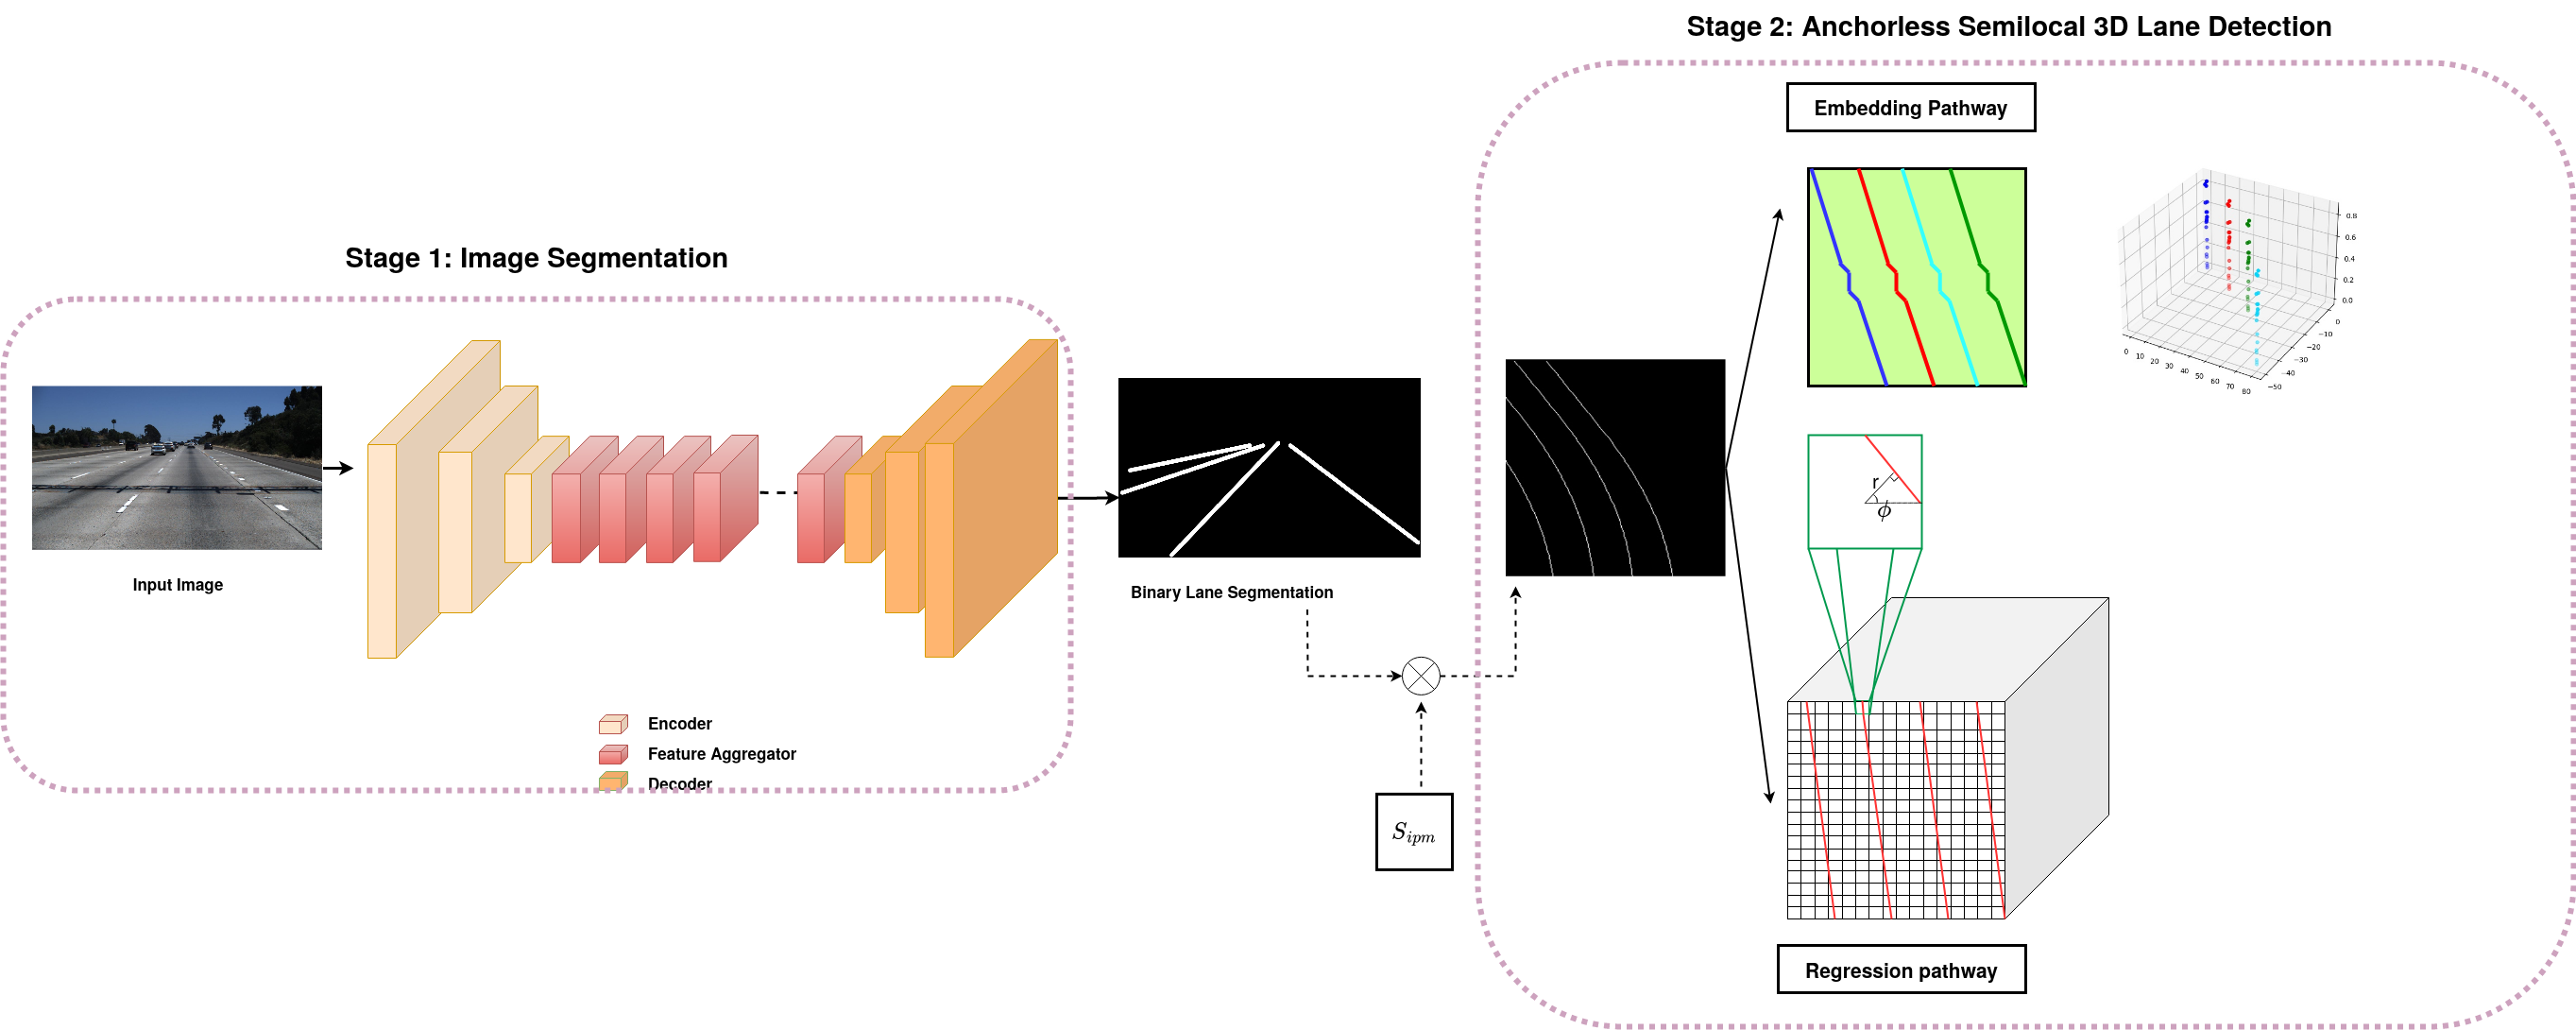
\includegraphics[width=\textwidth, height=7cm]{images/3DlaneAUXNet.png}
    \caption{Proposed dual stage semi-local anchor less 3D lane detection pipeline  \cite{guo2020gen}}
    \end{figure}
        
     As per the original idea of dual stage architecture proposed by \cite{guo2020gen}, the first stage is responsible for extracting features from a monocular image and obtaining a binary lane segmentation mask as an intermediate output. This binary segmentation mask is taken into birds-eye-view using projective transformation. Before feeding the top-view binary lane segmentation mask into the second stage of the network it is normalized. The second stage of the network is divided into two pathways named the regression pathway and the embedding pathway. The regression pathway is responsible for extracting geometric information for 3D lane curves. Inspired from \cite{DBLP:journals/corr/abs-2011-01535} we have used semi-local tile representation and predicted the full lane curve by decimating the whole lane curve into small lane segments and regress geometric parameters to represent that lane curve locally. To facilitate that the resulting bird-eye-view feature map is spatially divided into grids $G_{WxH}$ containing $WxH$ nonoverlapping patches which are also called tiles. Assuming that from every tile there passes a line segment and approximating that line segment as a straight line, the regression pathway regresses per tile $g_{ij}$ three parameters ie. relative distance to tile center $\widetilde{r_{ij}}$, line angle $\widetilde{\phi_{ij}}$ and height offset $\triangle \widetilde{Z_{ij}}$. Instead of flattening the feature map and employing fully connected layers to predict regression targets for each tile, the output from stage one is passed through a series of convolution layers which are processed in a non-overlapping or semi-overlapping way where the kernel stride is set equal to the tile size and in the later case half of the tile size. Such encoding is responsible for regressing the geometric parameters for representing a lane segment per each tile, the spatial size of the output feature map after this encoding is the same as $WxH$. Let's assume the spatial size of the output birds-eye-view feature map after the first stage is $(416,256)$ and diving this into a grid with each tile of size $(16,16)$, the resulting grid size will be $(26,16)$. Along with this the output size after the feature encoding is $(N, 13, H, W)$, here $(HxW) = (26x16)$ denoting the spatial size of the grid, and $13$ denotes the number of channels for representing the tile regression targets which will be more explained in the later sections. Each element in this grid at a particular index along the channel axes represents the regression values for that particular tile.
     
     In the embedding pathway, the normalized birds-eye lane binary segmentation mask is fed to a series of $1x1$ convolution layers which is responsible for learning global lane embeddings, inspired by \cite{DBLP:journals/corr/abs-1802-05591} mean-shift clustering is performed on the learned global lane embedding to complete multiple lane segments to complete lane curves. We learn an embedding vector $f_{ij}$ for each tile and using discriminative push-pull loss inspired from \cite{DBLP:journals/corr/abs-2011-01535} \cite{DBLP:journals/corr/abs-1802-05591} as an objective function to learn the global lane embeddings. The discriminative push-pull loss ensures that the embedding that belongs to the same line will stay close in the embedding space whereas embedding for tiles of different lanes will stay far from each other in the embedding space. 

    \subsection{Experimental setup: Approach 2}
    As we have discussed earlier in this approach we are trying to predict 3D lane line points semi-locally where the binary lane segmentation maps are transformed to a virtual top view and the regression pathway predicts the geometric parameters related to 3D lane curves and embedding learned via the embedding pathway is clustered to obtain lane line labels. Via each tile $g_{ij} \in G_{WxH}$ we are trying to approximate a lane segment and each tile will contribute one point to the 3D lane curve and we can trace the whole 3D lane curve. Below we will discuss in detail the generation of ground truth, loss functions used to learn the angle and height offsets, and how to generate a full 3D lane curve using the per tile predictions from the model. 
        \subsubsection{Ground Truth Creation}
        Following the idea proposed by \cite{DBLP:journals/corr/abs-2011-01535} that through each tile passes a single line segment and to approximate that line segment, we are trying to approximate it using a straight line. The regression pathway regresses per each tile $\widetilde{r_{ij}}$ lateral offset distance relative to tile center, line angle $\widetilde{\phi}_{ij}$, $\triangle{\widetilde{z_{ij}}}$ and this pathway also predicts a binary classification score $\widetilde{c_{ij}}$ denoting if a lane segment intersects that particular tile or not. 
        Ground-truth for the angle and distance offsets are computed by first projecting the ground-truth 3D lane points on the road plane in bird's eye view (BEV) and the resulting 2D lane curves are obtained in BEV. The resulting projected image is decimated into grids. Using the above-mentioned idea of approximating a lane curve by dividing it into small lane segments, we have used lane approximation algorithms like Hough Transform to obtain the $r_{ij}$ and $\phi_{ij}$. Thus representing the lane segment in the form of polar coordinates and this process is done for all the decimated tiles. The resulting line angle and distance offsets are calculated with respect to the origin at the center of each tile. To represent the line angle and distance offsets with respect to a global origin at the top-left corner of the image we have used Hesse normal form \footnotetext{\url{https://en.wikipedia.org/wiki/Hesse_normal_form}}. 
        
        
        Height offset $\triangle Z$ for each tile can be calculated by considering two scenarios in the figure below. 
        \begin{figure}[h]
        \centering
        \begin{subfigure}{0.4\textwidth}
        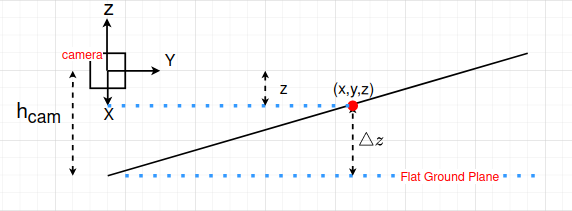
\includegraphics[width=1.2\linewidth, height=3cm]{images/delta_z_uphill.png} 
        \caption{}
        \label{fig:subim1}
        \end{subfigure}
        \begin{subfigure}{0.4\textwidth}
        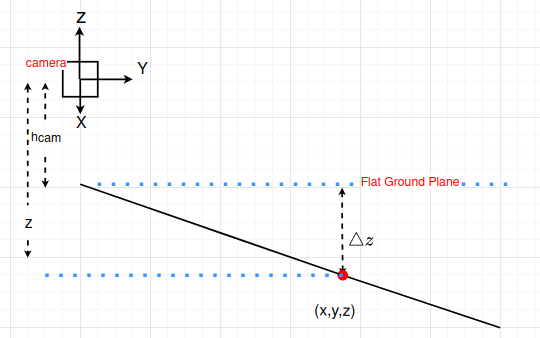
\includegraphics[width=1\linewidth, height=4cm]{images/delat_z_downhill.png}
        \caption{}
        \label{fig:subim2}
        \end{subfigure}
        
        \caption{Uphill and downhill driving scenario of an autonomous ego vehicle.}
        \label{fig:image2}
        \end{figure}
        
        
        \subsubsection{Loss Computation}
            For training, the position and angle offset $L1$ loss is used as an objective function. 
            
            \begin{equation}
                L^{Offsets}_{i,j} = \parallel \widetilde{r_{i,j}} - r_{i,j} \parallel_{1} + \parallel \triangle{\widetilde{z_{i,j}}} - \triangle{z_{i,j}} \parallel_{1} 
             \end{equation}
             
             The prediction of $\widetilde{\phi}_{ij}$ is carried out using a hybrid classification-regression schema proposed by \cite{}, where the classification of angle $\phi$ is done on the basis that it lies in one of $N_{\alpha}$ bins. Example, if we decide that each bin will have an interval of $36^{\circ}$ then there exists 10 bins, where $\alpha = \left\{\frac{2\pi}{N_{\alpha} } \cdot i \right\}^{N_{\alpha}}_{i =1} $. The network also regresses a vector $\triangle^{\alpha}$ which is responsible for addressing the residual offset related to bin classification. This bin estimation problem is optimized using a soft multi-label objective and the ground-truth probabilities for each bin is calculated via $ p^{\alpha} = [1 - \vert \frac{2\pi}{N_{\alpha}} \cdot i  - \phi  \vert \ \frac{2\pi}{N_{\alpha}} ]_{+}$.
             
             The resulting angle loss is the combination of classification and offset regression losses which can be defined as:
             \begin{equation}
                 L_{ij}^{Offsets} = \sum_{\alpha=1}^{N_{\alpha}}[p^{\alpha}_{ij} \cdot log \tilde{p^{\alpha}_{ij}} + (1 - p^{\alpha}_{ij}) + \delta^{\alpha}_{ij} \parallel   \tilde{\triangle^{\alpha}_{ij}} - \triangle^{\alpha}_{ij} \parallel_{1} ]
             \end{equation}
             
             In the above equation $\delta^{\alpha}_{ij}$ is an indicator function that is responsible for masking the bins for offset learning. 
             
             To train the lane tile probability $\widetilde{c_{ij}}$ is trained via binary cross entropy loss:
             \begin{equation}
                 L_{ij}^{score} = c_{ij} \cdot log \widetilde{c_{ij}} + (1 - c_{ij}) \cdot log
                    (1-  \widetilde{c_{ij}})
             \end{equation}
             
             Overall tile loss is the sum of the above-mentioned losses for all the tiles of the decimated grid:
             
            \begin{equation}
                L^{tiles} = \sum_{i,j \in WxH}(L^{score}_{ij} +c_{ij} \cdot L^{angle}_{ij} + c_{ij} \cdot L^{offsets}_{ij}  )
            \end{equation}
            
         a   To learn the global embeddings for lane curve clustering we have adopted the discriminative push-pull loss proposed in \cite{DBLP:journals/corr/abs-1802-05591} , \cite{DBLP:journals/corr/abs-1708-02551}. For each tile an embedding vector $f_{ij}$ is learned, the main idea behind using the discriminative push-pull loss is that embedding vectors that belong to the same lane would reside close to each other in the embedding space, and the vectors which belong to different lanes would reside apart. The above-mentioned discriminative push-pull loss is a sum of two losses:
            
            \begin{equation}
                L^{embedding} = L^{pull} + L^{push}
            \end{equation}
             
             \begin{equation}
                     L^{pull} = \frac{1}{C} \sum^{C}_{c=1}\frac{1}{N_{c}} \sum_{ij \in WXH}[ \delta_{ij}^{c} \parallel \mu_{c} - f_{ij}  \parallel - \triangle_{pull} ]_{+}^{2} 
             \end{equation}
             
             \begin{equation}
                 L^{push} =  \frac{1}{C(C -1)} \sum^{C}_{C_{A=1} } \sum^{C}_{C_{B=1}, C_{A} \not =C_{B}}[ \triangle_{push} - \parallel \mu_{CA} - \mu_{CB}\parallel ]_{+}^{2}
             \end{equation}
            
            Here $C$ is the number of lanes, $N_{c}$ denotes the number of tiles that belong to lane c, $\delta_{ij}^{c}$ denotes if tile $i,j$ belongs to lane c, $\mu_{c} = \frac{1}{N_{c}} \sum_{ij \in WXH } \delta^{c}_{ij} \cdot f_{ij}$ is the mean of embedding vector that belongs to lane $c$. $\triangle_{pull}$ and $\triangle_{pull}$ denote the maximum and minimum distance between the clusters. 
            
        \subsubsection{Final Output}
        
        Clustering is performed on the learned feature embedding and each tile contributes a point to the 3D lane curve. The predicted offsets and angles are converted to 3D lane line points by converting them from polar to Cartesian coordinates. Finally, the points are transformed from BEV to camera coordinate frame by rotating the points by  $-\theta_{cam}$ and subtracting by $h_{cam}$. 
        
        \begin{equation}
            \begin{bmatrix}\widetilde{x_{ij}}  \\\widetilde{y_{ij}} \\ \widetilde{z_{ij}}  \end{bmatrix} = \begin{bmatrix}1 & 0 & 0  \\ 0  & cos(\theta_{cam}) & sin(\theta_{cam}) \\ 0  & -sin(\theta_{cam}) & cos(\theta_{cam}) \end{bmatrix} \cdot \begin{bmatrix}\widetilde{r_{ij}} \cdot cos(\widetilde{\phi_{ij}})  \\\widetilde{r_{ij}} \cdot sin(\widetilde{\phi_{ij}})  \\ \widetilde{\triangle z_{ij}} - h_{cam} \end{bmatrix}
        \end{equation}
        

        \subsubsection{Evaluation Metrics}
        We have used the same evaluation schema as discussed in section 4.2.4. 
        
        \subsubsection{Implementation Details and Other Design Choices }
        For the first stage of this approach, we have used the best model obtained from our experimentation on binary lane segmentation which will be discussed in detail in later sections. BEV projection envelops $20.4m x 80m$ of the road and the BEV feature map is decimated to a grid, where each tile represents $16x16$ pixels, resulting in grid $G_{WXH}$ with W =16 and $H =26$. The resolution of each tile is $1.28m x 3m$ with $416x256$ as the spatial size of the BEV projection. Instead of predicting the camera height and pitch, we have used the values provided in the dataset itself.  The input image is
        resized to $(360x480)$ and normalized using Imagenet\cite{deng2009imagenet} mean and standard deviation values. ADAM with weight decay 1e − 4 is used as an optimizer to train our models. 0.001 is chosen as an initial learning rate and on top of that we have used ReduceLROnPlateu \footnote{\url{https://pytorch.org/docs/stable/generated/torch.optim.lr_scheduler.ReduceLROnPlateau.html#torch.optim.lr_scheduler.ReduceLROnPlateau}} as the learning rate scheduler with 0.75 as learning rate reduction factor, 3 as patience factor denotes the number of epochs to wait when the learning rate has to be reduced if there is no improvement in loss, 1e − 6 as the lowest learning rate managed by the scheduler. The model is trained with a batch size of 8 and training is carried out for 50 epochs. During training, the model is evaluated at every epoch and the results are visualized qualitatively and quantitatively using wandb \footnote{\url{https://wandb.ai}}. 0.1 and 3 are used as $\triangle_{pull}$ and $\triangle_{push}$, 0.3 is used as a threshold value on the predicted lane scores per tile before performing clustering.
        
\end{document}
